
\section{Extended Mean Field Training}
All classical training algorithms are a clever way of estimating expected values
over the distribution of the RBM. The algorithms are intrinsically stochastic
because random sample generation is used in all of them. We analyze now a completely
different approach by Gabriè~\cite{gabrie18training}, inspired by the mean-field
theory of the Ising model in Statistical Mechanics. The key idea is to notice that the
log-likelihood contains a term that is the free energy of the model. Moreover, the
algorithm is deterministic, since no random sample is needed.

The algorithm is essentially a different approach for computing the gradient. All other
considerations we have done in Section~\ref{subsec:general-gradient-rules} apply the same
also here. The weight decay is particularly important because the algorithm rely on the assumption
of weak interactions.

We present a pure mathematical derivation, highlighting the physics that inspired the
steps in {\bf \color{physics-blue}blue~boxes}, although it's not necessary to read them for
understating the procedure. We deal only with classical binary RBMs,
but the method can be generalized. We introduce also a few more notations in
{\bf \color{pink-notation}pink~boxes}.

%Include shortcuts
../emf-shortcuts.tex

\subsection{Introducing \(F\)}
\NotationBox{\vec{s}}{
  During the derivation, we use the more concise notation for vectors
  \[
    \vec{s} \coloneqq (\vec{v},\vec{h}),
  \]
  since many calculations we do hold both for hidden and visible layer.
  We use the index \(t\) for sums over \(\vec{s}\) components. In example
  \[
    \left|\vec{s}\right|^2 = \left|\vec{v}\right|^2 + \left|\vec{h}\right|^2
                           = \sum_{i=1}^{m} v_i^2 + \sum_{j=1}^{n} h_j^2
                           = \sumt s_t^2.
  \]
  We can also define vector indexed as \(\vec{s}\). For example a fictitious vector \(\vec{z}\)
  \[
    \vec{z} \coloneqq (\vec{z}^v,\vec{z}^h) \qquad
    \vec{s}\cdot\vec{z} = \vec{v}\cdot\vec{z}^v + \vec{h}\cdot\vec{z}^h
                        = \sum_{i=1}^{m} v_i z^v_i + \sum_{j=1}^{n} h_j z^h_j
                        = \sumt s_t z_t,
  \]
  and now should be completely clear how this notation works.
}

We recall from the previous section that the log-likelihood for an RBM is given by
\begin{equation} \label{eq:log-like-begiing-EMF}
  \log\likelihood{\vec{\theta}}{\vec{\bar{v}}}
    = \log\left(\sum_{\vec{h}} \exp\left[-E(\vec{\bar{v}},\vec{h})\right]\right)
      - \log\left(\sums \exp\left[-E(\vec{s})\right]\right)
\end{equation}
Once took the gradient the first term of this expression can be computed analytically,
as we have already seen. The second term leads to the expected values instead, so let's
focus on it. Let's define
\begin{equation} \label{eq:def-F}
  \FEn{\vec{q}}{\beta} \coloneqq - \frac{1}{\beta}
                           \log{\left[\sums \exp{\left(-\beta E(\vec{s}) + \beta \vec{q}\cdot\vec{s}\right)}\right]},
\end{equation}
so that the second term in equation~\eqref{eq:log-like-begiing-EMF} is exactly
\(\FEn{\vec{0}}{1}\).
Using these considerations the gradient of log-likelihood can be expressed in function of
\(F\). For example equation~\eqref{eq:logL-gradient-w-RBM} becomes
\[
  \ParDer{\log\likelihood{\vec{\theta}}{\vec{\bar{v}}}}{w_{i,j}} =
    \bar{v}_i \sigmoid{\sum_{i'=1}^m w_{i',j}\bar{v}_{i'}+c_j}
    +\ParDer{\left(\FEn{\vec{0}}{1}\right)}{w_{i,j}}.
\]
For now, we've only laid the foundation of the computation.

\PhysicsBox{What are \(F\) and \(\vec{q}\) in  physics?}{
  \(F\) is the Helmholtz free energy; \(\vec{q}\) the external magnetic field.
  
  One may ask now how can be \(\vec{q}\) the external fields if there are already \(b\)
  and \(c\) parameters in the energy \(E\) that do this role. The answer is that \(E\)
  is the microscopic Hamiltonian of the system, and of course \(b\) and \(c\) behave
  like a local parameter, but since they are a microscopic property, they haven't a 
  macroscopic thermodynamic quantity associated. Instead, since \(\vec{q}\) is controlled
  from the extern of the system, it can be treated as a thermodynamic variable.
  However, this does not mean that without \(\vec{q}\) the magnetization is null. The
  system can have ferromagnetic behavior, as we will see next sections.   
}

\subsection{Computing \(F\): \(\Gamma\) and \(A\)}
It's clear looking at equation~\eqref{eq:def-F} that \(F\) is at least \(C^\infty\)
in \(\vec{q}\). Moreover, it's a concave function, so \(-F\) is convex and so it's well
defined its Legendre~Transformation\footnote{The definition of Legendre Transformation
  used here it's more general than the one usually taught during courses. The best
  source I found at the moment is Wikipedia.}
\begin{equation}
  \Gam{\vec{m}}{\beta} \coloneqq \sup_{\vec{q}}{\left\{\vec{q}\cdot\vec{m}
                            - \left(-\FEn{\vec{q}}{\beta}\right)\right\}}
                       = \sup_{\vec{q}}{\left\{\vec{q}\cdot\vec{m}
                            + \FEn{\vec{q}}{\beta}\right\}}
                       = \qhat{\vec{m}}\cdot\vec{m} + \FEn{\qhat{\vec{m}}}{\beta}
\end{equation}
where
\[
  \qhat{\vec{m}} \coloneqq
  \argsup_{\vec{q}}{\left\{\vec{q}\cdot\vec{m} + \FEn{\vec{q}}{\beta}\right\}}.
\]
Since Legendre Transformation is involutive we have
\[
  -\FEn{\vec{q}}{\beta} = \sup_{\vec{m}}{\left\{\vec{q}\cdot\vec{m} - \Gam{\vec{m}}{\beta}\right\}},
\]
from which it's easy to see
\begin{equation*}
  -\beta \FEn{\vec{0}}{\beta} = -\beta \sup_{\vec{m}}{\left\{\vec{0}\cdot\vec{m} -
                                                             \Gam{\vec{m}}{\beta}\right\}}
                              = -\beta \sup_{\vec{m}}{\left\{-\Gam{\vec{m}}{\beta}\right\}}
                              = -\beta \inf_{\vec{m}}{\left\{\Gam{\vec{m}}{\beta}\right\}}
                              = -\beta \Gam{\vec{\hat{m}}}{\beta},
\end{equation*}
where 
\[
  \vec{\hat{m}} \coloneqq
  \arginf_{\vec{m}}{\left\{\Gam{\vec{m}}{\beta}\right\}}.
\]
Note in particular that the definitions of \(\qhat{\vec{m}}\) and \(\vec{\hat{m}}\) are quite
different. Our attention now shifts to \(\Gamma\) since if we compute and minimize it we
can get easily \(\FEn{\vec{0}}{1}\).

We prefer dealing with a different quantity rather than \(\Gamma\), so we define
\[
  A{\left[\vec{m};\beta\right]} \coloneqq -\beta \Gam{\vec{m}}{\beta}.
\]

\PhysicsBox{What are \(\Gamma\) and \(\vec{m}\) in  physics?}{
  \(\Gamma\) is the Gibbs free energy; \(\vec{m}\) is the magnetization.
  %TODO: explain much more.
}

\subsection{Computing \(A\)}
\NotationBox{\Fmean{\cdot}{\vec{q}}{\beta}}{
  If we call
  \[
    f{\left[\vec{q};\beta\right](\vec{s})} \coloneqq \exp{\left(-\beta E(\vec{s}) 
                                            + \beta \vec{q}\cdot\vec{s}\right)},
  \]
  we can write \(F\) as 
  \[
    \FEn{\vec{q}}{\beta} = -\frac{1}{\beta} \log{\left[\sums       
                                          f{\left[\vec{q};\beta\right](\vec{s})}\right]}.
  \]
  
  Given a generic operator \(O{(\vec{s})}\) it's well defined
  \[
    \Fmean{O}{\vec{q}}{\beta} =
      \frac{\sums O{(\vec{s})}f{\left[\vec{q};\beta\right](\vec{s})}}
           {\sum_{\vec{s'}}f{\left[\vec{q};\beta\right](\vec{s'})}}.
  \]
  \PhysicsBox{What is this in physical term?}{
    It's just the mean value  over the ensemble of the operator \(O\), written as
    function of independent variables \(\vec{q}\). 
  }
}
We would like to find a nicer expression for
\begin{equation} \label{eq:expression-for-A}
   A{\left[\vec{m};\beta\right]} =
    -\beta \left(\qhat{\vec{m}}\cdot\vec{m} + \FEn{\qhat{\vec{m}}}{\beta}\right).
\end{equation}
We can do the following observations on the expression 
\(-\beta \left(\vec{q}\cdot\vec{m} + \FEn{\vec{q}}{\beta}\right)\):
\begin{enumerate}[i]
  \item \(F\) is a smooth function of \(\vec{q}\), so the expression is smooth too and its
    extremes points are stationary;
  \item \(F\) is concave, so also the expression it is, since the term \(\qhat{\vec{m}}\cdot\vec{m}\)
    doesn't affect the convexity;
  \item given the previous two observations we can say that the expression has at most 1 stationary
    point and, if it exist, it must be a maximum.
\end{enumerate}
We can now write an equation for \(\qhat{\vec{m}}\)
\begin{align}
  \nonumber
  \vec{\nabla}_{\vec{q}} \Big(\vec{q}\cdot\vec{m} + \FEn{\vec{q}}{\beta}\Big)
    \bigg|_{\vec{q}=\qhat{\vec{m}}}&=0 \\
  \nonumber
  \vec{m} + \left.\ParDer{F}{\vec{q}}\right|_{\vec{q}=\qhat{\vec{m}}}&=0 \\
  \label{eq:m-s-mean}
  \vec{m} - \Fmean{\vec{s}}{\qhat{\vec{m}}}{\beta} = 0.
\end{align}
In other words, we can say that the function \(\qhat{\vec{m}}\) is the inverse of
magnetization function
\begin{equation}
  \label{eq:mean-magnetization}
  \vec{\bar{m}}{[\vec{q}]} \coloneqq \Fmean{\vec{s}}{\vec{q}}{\beta}.
\end{equation}
Starting from equation~\eqref{eq:expression-for-A} we can write
\begin{align}
  \nonumber
   A{\left[\vec{m};\beta\right]} &=
    \log{\left[\exp{\left(-\beta \vec{m}\cdot\qhat{\vec{m}}\right)}\right]}
      + \log{\left[\sums \exp{\left(-\beta E(\vec{s}) +  
                                        \beta\qhat{\vec{m}}\cdot\vec{s}\right)}\right]} \\
   \nonumber
   &= \log{\left[\exp{\left(-\beta \vec{m}\cdot\qhat{\vec{m}}\right)} \sums    
     \exp{\left(-\beta E(\vec{s}) + \beta\qhat{\vec{m}}\cdot\vec{s}\right)}\right]} \\
   \nonumber
   &= \log{\left[\sums\exp{\left(-\beta E(\vec{s}) +     
      \beta\qhat{\vec{m}}\cdot(\vec{s}-\vec{m})\right)}\right]} \\
   \label{eq:A-nicer-form}
   &= \log{\left[\sums\exp{\left(-\beta E(\vec{s}) +     
       \Lambd{\vec{m}}{\beta}\cdot(\vec{s}-\vec{m})\right)}\right]}
\end{align}
where we have defined the
\[
  \Lambd{\vec{m}}{\beta} \coloneqq \beta \qhat{\vec{m}}.
\]
\ExplainBox{The limit \(\beta \to 0\) for \(\vec{\lambda}\)}{
  Looking at its definition one could naively think that \(\Lambd{\vec{m}}{0}=0\).
  This is not true because by expanding \eqref{eq:mean-magnetization} one can see that\footnote{
    I'm bluffing; I've never done the calculation, but I'm confident  that what I'm saying it's true.}
 \[
  \left|\lim_{\beta\to0} \qhat{\vec{m}}\right| \to+\infty,
 \]
 so \(\vec{\lambda}\) can take finite values at \(\beta = 0\):
 \[\Lambd{\vec{m}}{0}\neq0.\]
 \PhysicsBox{Why this makes sense physically}{
   The function \(\qhat{\vec{m}}\) is answering the question ``what must be the field
   for having the magnetization equal to \(\vec{m}\)?''. The limit of \(\beta\to0\)
   corresponds to high temperatures, so the system it's much more disordered by thermal
   fluctuations. If we want to keep the magnetization fixed (so impose some kind of order)
   we have to use a  strong field to overcome the effect of temperature.
   It's natural that the field diverges.
 }
}
\NotationBox{\Gmean{\cdot}{\vec{q}}{\beta}}{
  In the analogy of the mean over \(F\):
  \[
  \gamma{\left[\vec{m};\beta\right](\vec{s})} \coloneqq \exp{\left(-\beta E(\vec{s}) +     
    \Lambd{\vec{m}}{\beta}\cdot(\vec{s}-\vec{m})\right)},
  \]
  and 
  \[
  \Gmean{O}{\vec{m}}{\beta} =
  \frac{\sums O{(\vec{s})}\gamma{\left[\vec{m};\beta\right](\vec{s})}}
  {\sum_{\vec{s'}}\gamma{\left[\vec{m};\beta\right](\vec{s'})}}.
  \]
  \PhysicsBox{What is this in physical term?}{
    It's just the mean value over the ensemble of the operator \(O\), written as
    a function of independent variables \(\vec{m}\).
  }
}
\subsection{Expansion of \(A\) around \(\beta=0\)}
Deal with the exact form of \(A\) given by equation~\eqref{eq:A-nicer-form} is hard,
so we expand around \(\beta = 0\) and use the truncated series for further steps.
Of course since in the end we need the result for \(\beta=1\) the more terms we keep, the better
it works. In our derivation, we use terms up to the third order.
\(A\) can be written as
\[
  A{\left[\vec{m};\beta\right]} \approx
    A{\left[\vec{m};0\right]} + 
    \beta \left.\ParDer{A{\left[\vec{m};\beta\right]}}{\beta}\right|_{\beta=0} +
    \frac{\beta^2}{2}
      \left.\frac{\partial^2A{\left[\vec{m};\beta\right]}}{\partial\beta^2}\right|_{\beta=0}+
    \frac{\beta^3}{6} 
      \left.\frac{\partial^3A{\left[\vec{m};\beta\right]}}{\partial\beta^3}\right|_{\beta=0}    
\]
Before going through the computation of the derivatives, we prove 2 useful lemmas.
\begin{lemma} \label{lem:lambda-t-zero}
  \(\Lambd{\vec{m}}{\beta}\) at \(\beta = 0\) is
  \[
    \lgtmz = \log{\left(m_t\right)} - \log{\left(1-m_t\right)}.
  \]
  \begin{proof}
    Let's write the component \(m_{\bar{t}}\) of the equation~\eqref{eq:m-s-mean}
    \[
      m_{\bar{t}} = \Fmean{s_{\bar{t}}}{\qhat{\vec{m}}}{0}
      = \frac{\sums s_{\bar{t}} e^{-\beta E(\vec{s}) + \beta \vec{\hat{q}}\cdot\vec{s}}}
             {\sum_{\vec{s'}}e^{-\beta E(\vec{s'}) + \beta \vec{\hat{q}}\cdot\vec{s'}}}
      = \frac{\sums s_{\bar{t}} e^{-\beta E(\vec{s}) + \Lambd{\vec{m}}{\beta}\cdot\vec{s}}}
             {\sum_{\vec{s'}}e^{-\beta E(\vec{s'}) + \Lambd{\vec{m}}{\beta}\cdot\vec{s'}}}
    \]
    Let's now fix \(\beta=0\)
    \begin{align*} \displaystyle
      m_{\bar{t}} &= \frac{\sums s_{\bar{t}} e^{\Lambd{\vec{m}}{\beta}\cdot\vec{s}}}
                          {\sum_{\vec{s'}}e^{\Lambd{\vec{m}}{\beta}\cdot\vec{s'}}} 
                   = \frac{\sums s_{\bar{t}} \prodt e^{\lgtmz s_t}}
                          {\sum_{\vec{s'}}\prodt e^{\lgtmz s'_t}} \\
                  &= \frac{\left(\sumstbar s_{\bar{t}}e^{\lgtbarmz s_{\bar{t}}}\right)
                           \prod_{t=1,t\neq{\bar{t}}}^{m+n}\left(\sumst e^{\lgtmz s_t}\right)}
                          {\prodt\sumstprim e^{\lgtmz {s'}_t}} \\
                  &= \frac{\sumstbar s_{\bar{t}}e^{\lgtbarmz s_{\bar{t}}}}
                          {\sumstbar e^{\lgtbarmz s_{\bar{t}}}}
                   = \frac{e^{\lgtbarmz}}{1+e^{\lgtbarmz}} = \sigmoid{\lgtbarmz}              
    \end{align*}
    Inverting the last equality gives the thesis.
  \end{proof}
\end{lemma}
\begin{lemma} \label{lem:operator-mean-gamma}
  Let \(O{(\vec{s})}\) an operator of the spins that can be written as a polynomial in the \(s_t\)
  variables, and \textbf{has at most degree 1 in each \(s_t\)}. Then
  \[
    \Gmean{O}{\vec{m}}{0} = O{(\vec{m})}.
  \]
  \ExplainBox{Why the hypotesis on the degree}{
    The key fact is that in our definition of RBM the nodes take values in \(\{0,1\}\), and both of these
    value has the property \(s_t^k = s_t \quad \forall k\in\mathbb{N}\), so when you write any power of
    a node value it's the same as writing the value itself. In example we 
    \[
      O{(\vec{s})} = 3s_1^2s_2 + 4s_1^3 + 5s_2^7 - 2 s_1 s_2^4 \equiv 4s_1+5s_2+s_1 s_2
    \]
    The energy instead is a proper operator on which apply the Lemma.
  }
  \begin{proof}
    Without losing generality we consider the operator
    \[O{(\vec{s})} = \prodt s_t.\]
    If we prove the thesis on this particular operator by linearity we can easily extend to all ones
    allowed by hypothesis.
    The computation is straightforward
    \begin{align*}
      \Gmean{O}{\vec{m}}{0} 
        &= \frac{\sums O{(\vec{s})} e^{\Lambd{\vec{m}}{\beta}\cdot(\vec{s}-\vec{m})}}
               {\sum_{\vec{s'}}e^{\Lambd{\vec{m}}{\beta}\cdot \cdot (\vec{s'}-\vec{m})}}
         = \frac{\sums \prodt s_t e^{\lgtmz \cdot (s_t-m_t)}}
                {\sum_{\vec{s'}} \prodt e^{\lgtmz \cdot ({s'}_t-m_t)}} \\
       &= \frac{\prodt \sumst s_t e^{\lgtmz \cdot (s_t-m_t)}}
               {\prodt \sumstprim e^{\lgtmz \cdot ({s'}_t-m_t)}}
        = \prodt \frac{e^{\lgtmz}}{1+e^{\lgtmz}} = \\
       &= \prodt \sigmoid{\lgtmz} = O{(\vec{m})}.
    \end{align*}
  \end{proof}
\end{lemma}
\subsubsection{Order 0}
The computation is easy
\begin{align*}
  A{\left[\vec{m};0\right]}
  &= \log{\left[\sums\exp{\left(\Lambd{\vec{m}}{0}\cdot(\vec{s}-\vec{m})\right)}\right]}
   = \log{\left[\sums\exp{\left(\sumt\lgtmz(s_t-m_t)\right)}\right]}\\
  &= \log{\left[\sums\prodt\exp{\left(\lgtmz(s_t-m_t)\right)}\right]}
   = \log{\left[\prodt\sumst\exp{\left(\lgtmz(s_t-m_t)\right)}\right]}\\
  &= \sumt\log{\left[e^{-\lgtmz m_t}(1+e^{\lgtmz})\right]}
   = \sumt\left[-\lgtmz m_t + \log{\left(1+e^{\lgtmz}\right)}\right]
\end{align*}
Now we can use the Lemma~\ref{lem:lambda-t-zero} and substitute \(\lgtmz\)
\begin{align*}
  A{\left[\vec{m};0\right]}
  &= \sumt\left[-\left(\log{\left(m_t\right)} - \log{\left(1-m_t\right)}\right) m_t
                + \log{\left(1+\frac{m_t}{1-m_t}\right)}\right] \\
  &= \sumt\left[-\log{\left(m_t\right)}m_t + \log{\left(1-m_t\right)}m_t
                - \log{\left(1-m_t\right)}\right] \\
  &= -\sumt\left[\log{\left(m_t\right)}m_t + \log{\left(1-m_t\right)}(1-m_t)\right] \\
  &= \sumt S_2{(m_t)}
\end{align*}
where \(S_2{(\cdot)}\) is the entropy of a binary distribution.
\PhysicsBox{Order 0 in physics}{
  The order 0 is the total entropy of the system when spins are not correlated.
}

\subsubsection{First order} \label{subsec:order-1-A}
We compute the derivative starting from equation~\eqref{eq:A-nicer-form}
\begin{align*}
  \left.\ParDer{A{\left[\vec{m};\beta\right]}}{\beta}\right|_{\beta=0}
  &= \left.
    \frac{
      \sums\left(-E{(\vec{s})}+\ParDer{\Lambd{\beta}{\vec{m}}}{\beta}\cdot(\vec{s}-\vec{m})\right)\GammaExp{}
    }{
      \sum_{\vec{s'}}\GammaExp{'}
    }\right|_{\beta=0}\\
  &= \Gmean{-E{(\vec{s})}}{\vec{m}}{0} +
     \left.\ParDer{\Lambd{\beta}{\vec{m}}}{\beta}\right|_{\beta=0}\cdot\Gmean{\vec{s}-\vec{m}}{\vec{m}}{0}\\
  &= -E{(\vec{m})}
\end{align*}
In the last equality we have used the Lemma~\ref{lem:operator-mean-gamma}.
\PhysicsBox{Order 1 in physics}{
  First order is the total energy of the system (multiplied by \(\beta\) where spins are set equal
  to the mean magnetization.
}

\subsubsection{Second order}
Let's begin with a lemma that we use later in the calculation.
\begin{lemma} \label{lem:first-derivative-lambda}
  The derivative of \(\Lambd{\vec{m}}{\beta}\) at \(\beta = 0\) is
  \begin{align*}
    \left.\ParDer{\lvim{\beta}}{\beta}\right|_{\beta=0} &= -\sum_{j=1}^n w_{i,j}m^h_j-b_i\\
    \left.\ParDer{\lhjm{\beta}}{\beta}\right|_{\beta=0} &= -\sum_{i=1}^m w_{i,j}m^v_i-c_j
  \end{align*}
  \begin{proof}
    Let's consider the quantity
    \begin{align*}
      \ParDer{}{\vec{m}}\left(\left.\ParDer{A{\left[\vec{m};\beta\right]}}{\beta}\right|_{\beta=0}\right)
      &= \left.\left(\ParDer{}{\beta}\ParDer{A{\left[\vec{m};\beta\right]}}{\vec{m}}\right)\right|_{\beta=0}
      = \left.\left(\ParDer{}{\beta}\Gmean{-\Lambd{\vec{m}}{\beta}}{\vec{m}}{\beta}\right)\right|_{\beta=0}
      = -\left.\ParDer{\Lambd{\vec{m}}{\beta}}{\beta}\right|_{\beta=0}
    \end{align*}
    where we were able to exchange derivative because \(A\) is smooth.
    We can compute the same quantity explicitly using the result obtained in
    section~\ref{subsec:order-1-A}
    \[
      \ParDer{}{\vec{m}}\left(\left.\ParDer{A{\left[\vec{m};\beta\right]}}{\beta}\right|_{\beta=0}\right)
      = -\ParDer{E{(\vec{m})}}{\vec{m}}.
    \]
    The thesis can be obtained by explicitly write the vector components.
    \PhysicsBox{The idea behind this proof}{
      Essentially what we are doing when we exchange derivatives in the first passage is using 
      a \emph{Maxwell relation} on the potential \(\Gamma\) (here we use \(A\) for convenience).
    }
  \end{proof}
\end{lemma}
Going back to the main calculation, we can start again from equation~\eqref{eq:A-nicer-form} after little calculations we get
\begin{align*}
  \left.\frac{\partial^2A{\left[\vec{m};\beta\right]}}{\partial\beta^2}\right|_{\beta=0}
  &= \Gmean{
       \left.\frac{\partial^2\vec{\lambda}{\left[\vec{m};\beta\right]}}{\partial\beta^2}\right|_{\beta=0}
         \cdot (\vec{s}-\vec{m})
       +\left(-E{(\vec{s})} +   
          \left.\ParDer{\Lambd{\beta}{\vec{m}}}{\beta}\right|_{\beta=0}\cdot(\vec{s}-\vec{m})\right)^2
     }{\vec{m}}{0}+\\
  &\quad+ \Gmean{
          -E{(\vec{s})}+\left.\ParDer{\Lambd{\beta}{\vec{m}}}{\beta}\right|_{\beta=0}\cdot(\vec{s}-\vec{m})
       }{\vec{m}}{0}^2 \\
  &= \Gmean{
       \left(-E{(\vec{s})} +   
        \left.\ParDer{\Lambd{\beta}{\vec{m}}}{\beta}\right|_{\beta=0}\cdot(\vec{s}-\vec{m})\right)^2
     }{\vec{m}}{0} - \left[E{(\vec{m})}\right]^2
\end{align*}
Let's focus on the term inside the bracket: we can use Lemma~\ref{lem:first-derivative-lambda}
to evaluate the derivative of \(\vec{\lambda}\) (only in these few passages we use Einstein notation
for summed indexes)
\begin{align*}
  -E{(\vec{s})} + \left.\ParDer{\Lambd{\beta}{\vec{m}}}{\beta}\right|_{\beta=0}\cdot(\vec{s}-\vec{m})
  &= v_iw_{i,j}h_j +b_iv_i+c_jh_j - (v_i-\mvi)(w_{i,j}\mhj +b_i) - (\mvi w_{i,j}+c_j)(h_j-\mhj) \\
  &= v_iw_{i,j}h_j - v_i w_{i,j} \mhj - \mvi w_{i,j} h_j + \mvi w_{i,j} \mhj - E{(\vec{m})}\\
  &= w_{i,j} (v_i-\mvi)(h_j-\mhj) - E{(\vec{m})}
\end{align*}
We can substitute this result in the expression above
\begin{align*}
  &\left.\frac{\partial^2A{\left[\vec{m};\beta\right]}}{\partial\beta^2}\right|_{\beta=0}=\\
  &\qquad= \Gmean{
      \sum_{i,j=1}^{m,n}\sum_{p,q=1}^{m,n} w_{i,j} w_{p,q}(v_i-\mvi)(h_j-\mhj)(v_p-m_p^v)(h_q-m_q^h)
      +2E{(\vec{m})}\sum_{i,j=1}^{m,n}w_{i,j}(v_i-\mvi)(h_j-\mhj)
    }{\vec{m}}{0}
\end{align*}
As a direct consequence of Lemma~\ref{lem:operator-mean-gamma} if a term is proportional to \(s_t-m_t\)
it cancels out when averaged on \(\gamma\). This fact makes the second term of the expression go away,
and in the first only the ones with \(i=p\) and \(j=q\) survive
\begin{align*}
  \left.\frac{\partial^2A{\left[\vec{m};\beta\right]}}{\partial\beta^2}\right|_{\beta=0}
    &=\Gmean{\sum_{i,j=1}^{m,n} w_{i,j}^2\left(v_i-\mvi\right)^2\left(h_j-\mhj\right)^2}{\vec{m}}{0} \\
    &=\Gmean{\sum_{i,j=1}^{m,n} w_{i,j}^2\left(v_i^2 -2v_i\mvi+\mvisq\right)\left(h_j^2-2h_j\mhj +\mhjsq\right)}{\vec{m}}{0}\\
    &\equiv\Gmean{\sum_{i,j=1}^{m,n} w_{i,j}^2\left(v_i-2v_i\mvi+\mvisq\right)\left(h_j-2h_j\mhj +\mhjsq\right)}{\vec{m}}{0}\\
    &=\sum_{i,j=1}^{m,n} w_{i,j}^2\left(\mvi-\mvisq\right)\left(\mhj-\mhjsq\right)
\end{align*}
where we used the equivalence \(s_t^2 \equiv s_t\), and the Lemma~\ref{lem:operator-mean-gamma}
for computing the average.

\subsubsection{Third order}
The calculation of the third order is not too different from the second order, it only needs more
steps and an expression for the second derivative of \(\vec{\lambda}\) that can be derived easily.
We don't report the full calculation, but only the result, taken from \cite{gabrie18training}
\[
  \left.\frac{\partial^3A{\left[\vec{m};\beta\right]}}{\partial\beta^3}\right|_{\beta=0}
  = 4 \sum_{i,j=1}^{m,n} w_{i,j}^3\left(\mvi-\mvisq\right) \left(\frac{1}{2}-\mvi\right)
                                  \left(\frac{1}{2}-\mhj\right) \left(\mhj-\mhjsq\right).
\]
Alternatively, this result (and also higher and lower orders) can be computed using the formalism
developed in \cite{georges1991expand}, which makes the calculations much easier.
\ExplainBox{Why don't we use order higher than 3}{
  The reason is that computing higher orders is so computationally expensive that it is
  not worth it. The \(k\)-th order can be thought of as the sum over the \emph{strongly irreducible connected
  sub-graph} of the RBM, with \emph{\(k\) arcs} and where edges can be considered multiple
  times\footnote{
    This picture does not give coefficients (that still require a full calculation to be computed),
     but it only helps to double-check the calculations.
  }.
  In this picture the orders we have computed are
  \begin{itemize}
    \item order 0 are all the single nodes;
      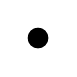
\begin{tikzpicture}
  \node[circle,fill=black,inner sep=2.5pt,draw] (a) at (180:1cm) {};
\end{tikzpicture}

    \item order 1 are all the pairs directly connected, with the corresponding edge;
      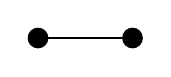
\begin{tikzpicture}
  \node[circle,fill=black,inner sep=2.5pt,draw] (a) at (180:0.6cm) {};
  \node[circle,fill=black,inner sep=2.5pt,draw] (b) at (0:0.6cm) {};
  \draw[thick] (a) -- (b);
\end{tikzpicture}
   
    \item order 2 are again all the pairs directly connected, but with the corresponding 	
      edge considered 2 times; 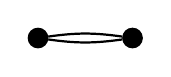
\begin{tikzpicture}
  \node[circle,fill=black,inner sep=2.5pt,draw] (a) at (180:0.6cm) {};
  \node[circle,fill=black,inner sep=2.5pt,draw] (b) at (0:0.6cm) {};
  \draw[thick] (a) edge[bend left=8] (b);
  \draw[thick] (a) edge[bend right=8] (b);
\end{tikzpicture}

    \item order 3 can have 2 different topologies \emph{a priori}:
      \begin{itemize}
        \item pairs directly connected with the corresponding edge considered 3 times;
          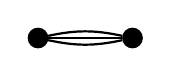
\begin{tikzpicture}
  \node[circle,fill=black,inner sep=2.5pt,draw] (a) at (180:0.6cm) {};
  \node[circle,fill=black,inner sep=2.5pt,draw] (b) at (0:0.6cm) {};
  \draw[thick] (a) edge[bend left=12] (b);
  \draw[thick] (a) edge[bend right=12] (b);
  \draw[thick] (a) -- (b);
\end{tikzpicture}

        \item triangles;\\
          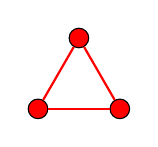
\begin{tikzpicture}
  \node[circle,fill=red,inner sep=2.5pt,draw] (a) at (90:0.6cm) {};
  \node[circle,fill=red,inner sep=2.5pt,draw] (b) at (210:0.6cm) {};
  \node[circle,fill=red,inner sep=2.5pt,draw] (c) at (330:0.6cm) {};
  \draw[red, thick] (a) -- (b);
  \draw[red, thick] (b) -- (c);
  \draw[red, thick] (c) -- (a);
\end{tikzpicture}

      \end{itemize}
      But triangles are not allowed by the RBM's topology, since there aren't edges between
      nodes in the same layer.
  \end{itemize}
  So to compute the first 3 orders we have to sum only on the edges, that it is still reasonable.
  The fourth order instead (and also orders above) has a \emph{quadrilateral} topology that does not
  go away, so it requires a sum on all possible pairs of edges, which is too much.\\
  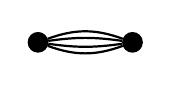
\begin{tikzpicture}
  \node[circle,fill=black,inner sep=2.5pt,draw] (a) at (180:0.6cm) {};
  \node[circle,fill=black,inner sep=2.5pt,draw] (b) at (0:0.6cm) {};
  \draw[thick] (a) edge[bend left=20] (b);
  \draw[thick] (a) edge[bend left=8] (b);
  \draw[thick] (a) edge[bend right=8] (b);
  \draw[thick] (a) edge[bend right=20] (b);
\end{tikzpicture}

  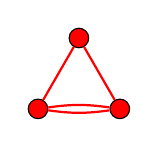
\begin{tikzpicture}
  \node[circle,fill=red,inner sep=2.5pt,draw] (a) at (90:0.6cm) {};
  \node[circle,fill=red,inner sep=2.5pt,draw] (b) at (210:0.6cm) {};
  \node[circle,fill=red,inner sep=2.5pt,draw] (c) at (330:0.6cm) {};
  
  \draw[red, thick] (a) -- (b);
  \draw[red, thick] (b) edge[bend left=8]  (c);
  \draw[red, thick] (b) edge[bend right=8] (c);
  \draw[red, thick] (c) -- (a);
\end{tikzpicture}
  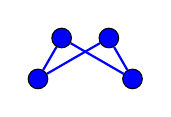
\begin{tikzpicture}
  \node[circle,fill=blue,inner sep=2.5pt,draw] (a) at (180:0.6cm) {};
  \node[circle,fill=blue,inner sep=2.5pt,draw] (b) at (0:0.6cm) {};
  \node[circle,fill=blue,inner sep=2.5pt,draw] (c) at (60:0.6cm) {};
  \node[circle,fill=blue,inner sep=2.5pt,draw] (d) at (120:0.6cm) {};

  \draw[blue, thick] (a) -- (c);
  \draw[blue, thick] (b) -- (c);
  \draw[blue, thick] (a) -- (d);
  \draw[blue, thick] (b) -- (d);
\end{tikzpicture}

  
  %In \cite{georges1991expand} there are some drawings that can help in understanding the picture
  %we have described.
}

\subsubsection{Put all the pieces together}
Now we have computed all the orders that we need we can write
\begin{align*}
A{\left[\vec{m}^v, \vec{m}^h;\beta\right]} &\approx
  -\sum_{i=1}^{m}\left[\log{\left(\mvi\right)}\mvi + \log{\left(1-\mvi\right)}(1-\mvi)\right]
  -\sum_{j=1}^{n}\left[\log{\left(\mhj\right)}\mhj + \log{\left(1-\mhj\right)}(1-\mhj)\right]\\
  &\quad+\beta \sum_{i,j=1}^{m,n}\mvi w_{i,j} \mhj +\beta\sum_{i=1}^{m} b_i\mvi +\beta\sum_{j=1}^{m} c_j\mhj\\
  &\quad+\frac{\beta^2}{2}
  \sum_{i,j=1}^{m,n} w_{i,j}^2\left(\mvi-\mvisq\right)\left(\mhj-\mhjsq\right)\\
  &\quad+\frac{2}{3}\beta^3 
    \sum_{i,j=1}^{m,n} w_{i,j}^3\left(\mvi-\mvisq\right) \left(\frac{1}{2}-\mvi\right)
    \left(\frac{1}{2}-\mhj\right) \left(\mhj-\mhjsq\right),
\end{align*}
that is the approximated formula we will use to do our further calculations.

\subsection{Estimation of the log-likelihood gradient}
The quantity we are interested in is \(\FEn{\vec{0}}{1}\) that can be calculated by minimizing \(\Gam{\vec{m}}{1}\).
First of all, we set \(\beta=1\) as RBM distributions, and using the approximation
on \(A\) we write
\begin{align*}
  \Gam{\vec{m}^v, \vec{m}^h}{1} &\approx
    \quad\sum_{i=1}^{m}\left[\log{\left(\mvi\right)}\mvi + \log{\left(1-\mvi\right)}(1-\mvi)-b_i\mvi\right]\\
    &\quad+\sum_{j=1}^{n}\left[\log{\left(\mhj\right)}\mhj+\log{\left(1-\mhj\right)}(1-\mhj)-c_j\mhj\right]\\
    &\quad-\sum_{i,j=1}^{m,n}\Bigg[
      \mvi w_{i,j}\mhj
      +\frac{1}{2}w_{i,j}^2\left(\mvi-\mvisq\right)\left(\mhj-\mhjsq\right)+\\
      &\qquad\qquad\quad+\frac{2}{3}w_{i,j}^3\left(\mvi-\mvisq\right)\left(\frac{1}{2}-\mvi\right)\left(\frac{1}{2}-\mhj\right)
        \left(\mhj-\mhjsq\right)
    \Bigg]
\end{align*}
We use this equation both for finding the minimum \(\vec{\hat{m}}\), and the to compute gradient.

\subsubsection{Equation for the minimum of \(\Gamma\)}
Since \(\Gamma\) is convex and smooth we have an easy equation for \(\vec{\hat{m}}\)
\[
  \left.\ParDer{\Gam{\vec{m}}{1}}{\vec{m}}\right|_{\vec{m}=\vec{\hat{m}}}=0.
\]
Let's compute the gradient with respect to \(\mvi\), the case \(\mhj\) is  the same.
\begin{align*}
  \left.\ParDer{\Gam{\vec{m}}{1}}{\mvi}\right|_{\vec{m}=\vec{\hat{m}}}
    &= \log\left(\hmvi\right) + 1 - \log\left(1-\hmvi\right) - 1 - b_i \\
    &\quad-\sum_{j=1}^n\bigg[w_{i,j}\hmhj
      +\frac{1}{2}w^2_{i,j}\left(1-2\hmvi\right)\left(\hmhj-\hmhjsq\right) \\
      &\qquad\qquad+\frac{2}{3}w_{i,j}^3\left(3\hmvisq-3\hmvi+\frac{1}{2}\right)\left(\frac{1}{2}-\hmhj\right)
      \left(\hmhj-\hmhjsq\right)\bigg].
\end{align*}
Now we notice that
\[
  \log{\left(\frac{y}{1-y}\right)} = x \quad \implies \quad y = \sigmoid{x},
\]
and  applying to the equation above we get the \emph{consistency relations} for the magnetization
\begin{align}
  \label{eq:converge-hmvi}
  \hmvi&=\sigmoid{b_i + \sum_{j=1}^n\left[w_{i,j}\hmhj+
           \left(\hmhj-\hmhjsq\right)\left(w^2_{i,j}\left(\frac{1}{2}-\hmvi\right)
           +w_{i,j}^3\left(2\hmvisq-2\hmvi+\frac{1}{3}\right)\left(\frac{1}{2}-\hmhj\right)
           \right)\right]}\\
  \label{eq:converge-hmhj}
  \hmhj&=\sigmoid{c_j + \sum_{i=1}^m\left[w_{i,j}\hmvi+
           \left(\hmvi-\hmvisq\right)\left(w^2_{i,j}\left(\frac{1}{2}-\hmhj\right)
           +w_{i,j}^3\left(2\hmhjsq-2\hmhj+\frac{1}{3}\right)\left(\frac{1}{2}-\hmvi\right)
           \right)\right]}
\end{align}
Solving these equations gives us \(\vec{\hat{m}}\) to be used when evaluating the gradient.
Attention must be paid since the fixed point of these equations it's not unique, but only
one is the  global minimum.
\MyIdeaBox{Solving these equations}{
  In the article \cite{gabrie18training}, the suggested method for solving these equations 
  is just to start from a random guess of \(\vec{m}\), and then iterate an appropriate
  number of times (in the article is 3-30). After these iterations we are quite confident
  that \(\vec{m}\) is decently converged.
  
  I'm quite convinced that this is far from the optimal solution. Maybe a smarter
  implementation of solutions finding can speed up the algorithm noticeably.
}

\subsubsection{Gradient respect to parameters}
To complete our update rule we have to calculate
\[
  \ParDer{\left(\FEn{\vec{0}}{1}\right)}{\vec{\theta}} =
  \ParDer{\left(\Gam{\vec{\hat{m}}}{1}\right)}{\vec{\theta}}
\]  
The calculation is straightforward using the expression above of \(\Gamma\)
\begin{align*}
  \ParDer{\left(\Gam{\vec{\hat{m}}}{1}\right)}{b_i} &= -\hmvi\\
  \ParDer{\left(\Gam{\vec{\hat{m}}}{1}\right)}{c_j} &= -\hmhj\\
  %
  \ParDer{\left(\Gam{\vec{\hat{m}}}{1}\right)}{w_{i,j}}
    &=-\Bigg[\hmvi\hmhj +w_{i,j}\left(\hmvi-\hmvisq\right)\left(\hmhj-\hmhjsq\right)+\\
    &\qquad+2w_{i,j}^2\left(\hmvi-\hmvisq\right)\left(\frac{1}{2}-\hmvi\right)\left(\frac{1}{2}-\hmhj\right)
      \left(\hmhj-\hmhjsq\right)\Bigg]
\end{align*}

\subsection{Persistent EMF training}
Using the same idea of PCD-\(k\), we can implement an algorithm that keeps track of the previous estimated value of \(\vec{m}\), and  use it as initial parameter to converge the equations~\eqref{eq:converge-hmvi}~and~\eqref{eq:converge-hmhj}.
